\documentclass[11pt]{article}
\usepackage{amsfonts}%For Maths fonts.
\usepackage{amssymb}%For math symbols.
\usepackage{amsmath}%For the math.
\usepackage{graphicx}%For the image.
\graphicspath{ ./} 
\usepackage{tikz}
\usepackage{float}
\usepackage{hyperref} 
\usepackage{listings}
\usepackage{color}
\usepackage{csvsimple}
\usepackage{dirtree}
\usepackage{graphicx}
\definecolor{dkgreen}{rgb}{0,0.6,0}
\definecolor{gray}{rgb}{0.5,0.5,0.5}
\definecolor{mauve}{rgb}{0.58,0,0.82}

\lstset{frame=tb,
	language=python,
	aboveskip=3mm,
	belowskip=3mm,
	showstringspaces=false,
	columns=flexible,
	basicstyle={\small\ttfamily},
	numbers=none,
	numberstyle=\tiny\color{gray},
	keywordstyle=\color{blue},
	commentstyle=\color{dkgreen},
	stringstyle=\color{mauve},
	breaklines=true,
	breakatwhitespace=true,
	tabsize=3
}

\usetikzlibrary{shapes.geometric, arrows}%For the borders and shapes.
\begin{document}
	\begin{titlepage}
		\begin{flushleft}
			
			\bf CS7.301
			\hfill
			\bfseries 2$^{nd}$ April, 2020
		\end{flushleft}
		\begin{center}
			\line(1,0){300}\\
			[5mm]
			\huge{\bfseries MDL Assignment-3}\\
			\line(1,0){300}\\
			[12cm]
		\end{center}
		\begin{flushright}
			{
				\line(1,0){270}\\
				\large  Vikrant Dewangan, Roll No.- 2018111024\\  Mohammad Nomaan Qureshi,
				Roll No.- 2018111027
				\line(1,0){270}\\	
			}
		\end{flushright}
	\end{titlepage}
	\newpage
	\tableofcontents
	\newpage
	\section{File Structure}
	Upon running the file \textit{solution.py}, we get 
	\dirtree{%
		.1 team\.71.
		.2 report.pdf: contains report.
		.2 client.py: contains necessary functions for server.
		.2 set\_cur\_state.py: contains necessary functions for vectors.
		.2 solution.py: main solution.
		.2 trace\_71.txt: trace obtained.
	}
	\section{Problem Statement}
	Given coefficients of vectors corresponding to over-fit model, apply Genetic Algorithm (G.A) to reduce over-fitting. 
	\\
	\textbf{\emph{Input}}:
	\begin{align*}
		\bar{v}_{overfit}&= [-0.00016927573251173823, 0.0010953590656607808,
		\\ & \hspace{0.5cm} 0.003731869524518327, 0.08922889556431182,
		\\ & \hspace{0.5cm} 0.03587507175384199, -0.0015634754169704097,
		\\ & \hspace{0.5cm} -7.439827367266828e-05, 3.7168210026033343e-06, 
		\\ & \hspace{0.5cm} 1.555252501348866e-08, -2.2215895929103804e-09, 
		\\  & \hspace{0.5cm}2.306783174308054e-11]
	\end{align*}
	Given a query server to allow for submission of weights ($w_i$), the following is returned for each query - 
	\begin{align*}
		M.S.E &= \frac{\sum_{x\in data} \big(y - f\big(x\big)\big)^{2}}{N}
	\end{align*}
	where $f\big(x\big)$ is calculated using the weights submitted $[w_1,w_2 \ldots w_{10}]$ - 
	\begin{align*}
		f\big(x\big) &= \sum_{i=1}^{10} w_i\cdot x_i
	\end{align*}
	\\	
	\textbf{\emph{Output}}:	
	A set of weights $[w_1,w_2 \ldots w_{10}]$ corresponding to best-fit under the conditions- 
	\begin{align*}
		|w_i| &\leq 10
	\end{align*}
	\section{Algorithm Definition}
	Our Genetic Algorithm consists of 4 steps - 
	\begin{enumerate}
		\item \textbf{Initialisation of Population}:\\
		Each generation contains 5 vectors. This is chosen from previous set of population or derived initially randomly.After the algorithm runs, this population is instead chosen from the already saved state in \textit{current\_state.pkl}.
		\begin{center}
			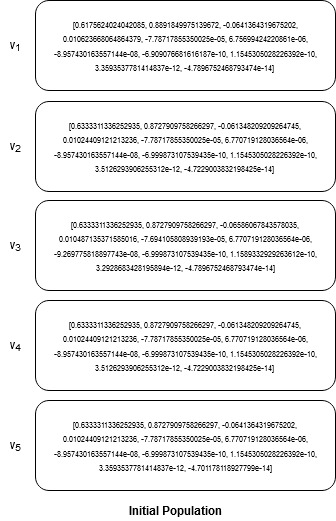
\includegraphics[width=0.6\linewidth]{population.jpg}
			\\
			\textit{population.jpg}
		  \end{center}
		\item \textbf{Fitness Function}:\\
		The best three of each iteration survive
and give birth to next generation. We chose training error to be out fitness function.
\begin{center}
	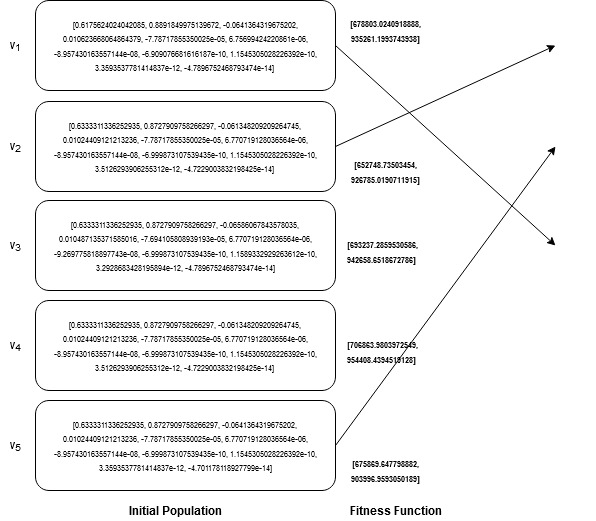
\includegraphics[width=\linewidth]{fitness.jpg}
	\\
	\textit{fitness.jpg}
\end{center}
	\item \textbf{Selection} \\
	Since we have used training error as our fitness function , the best 3 vectors are \textbf{deterministically} chosen from 
	the population. This is where we differ from the normal Genetic Algorithm that the selection is not random.
	\begin{center}
		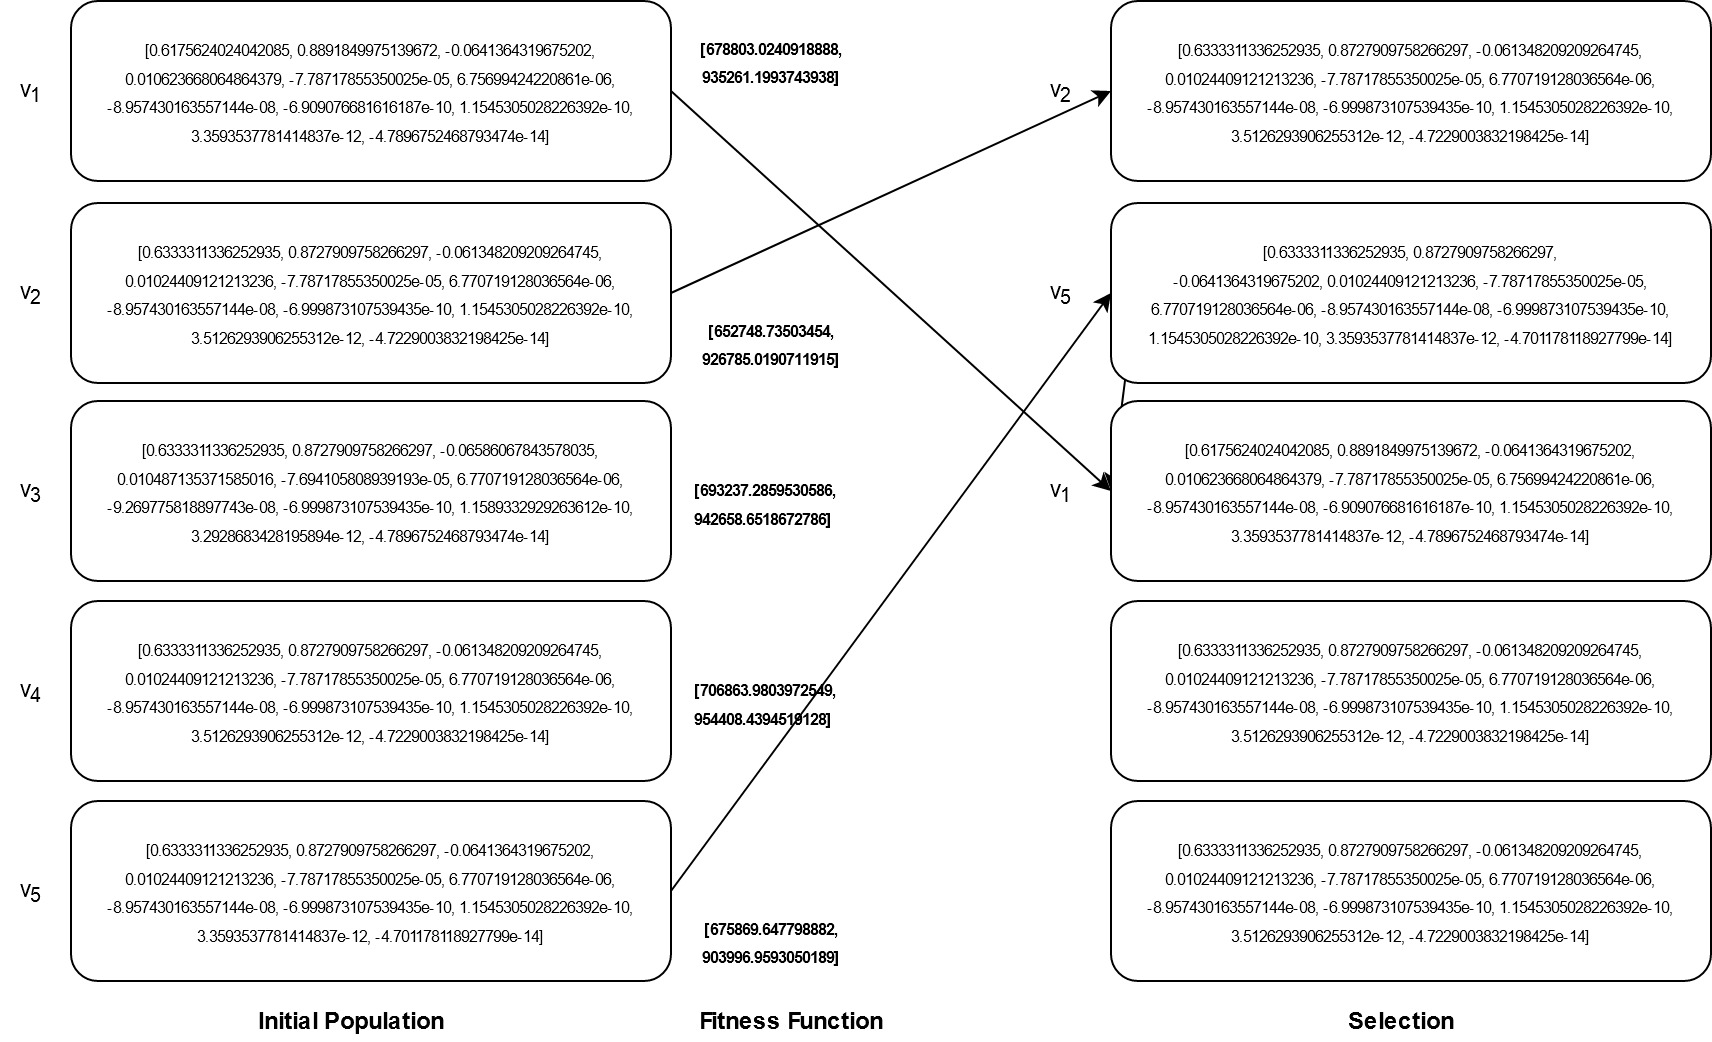
\includegraphics[width=\linewidth,height=10cm]{selection2.jpg}
		\\
		\textit{selection.jpg}
	\end{center}
	  So if A, B, C, D, E are in sorted order of
	  their fitness function then A, B, C
	  survive.The best three of each iteration survive
	  and give birth to next generation.
	\item \textbf{Crossover with Mutation} \\
	\textbf{Crossover} \\
	We did a probabilistic cross over which is
explained below. 

A is best vector and B is second best vector, then let Crossover vector be $C$.
\[
	C_i = \left.
	\begin{cases}
	  A_i, & \text{with } p_i = 0.6  \\
	  B_i, & \text{with } q_i = 0.4 
	\end{cases}
	\right\}
  \]
\textbf{Mutation}
The mutation was also probabilistic. Let $M$ be the new mutation vector. 
\[
	M_i = \left.
	\begin{cases}
	  A_i, & \text{with } p_i = 0.6  \\
	  \in (0.95*A_i,1.05*A_i), & \text{with } q_i = 0.4 
	\end{cases}
	\right\}
  \]

	Suppose the chosen population was A,B and C (with A giving the best value in fitness function, B the next best and then C).
	 The new vectors are
	\begin{itemize}
		\item	A-B (Crossover with Mutation).
		\item 	A-C (Crossover with Mutation).
		\item 	B-C (Crossover with Mutation).
		\item 	A with mutations: This is A with the following mutation.
		\item 	A without any mutation: This is just plain A without any mutation.
	\end{itemize}
	\end{enumerate}
	\begin{center}
		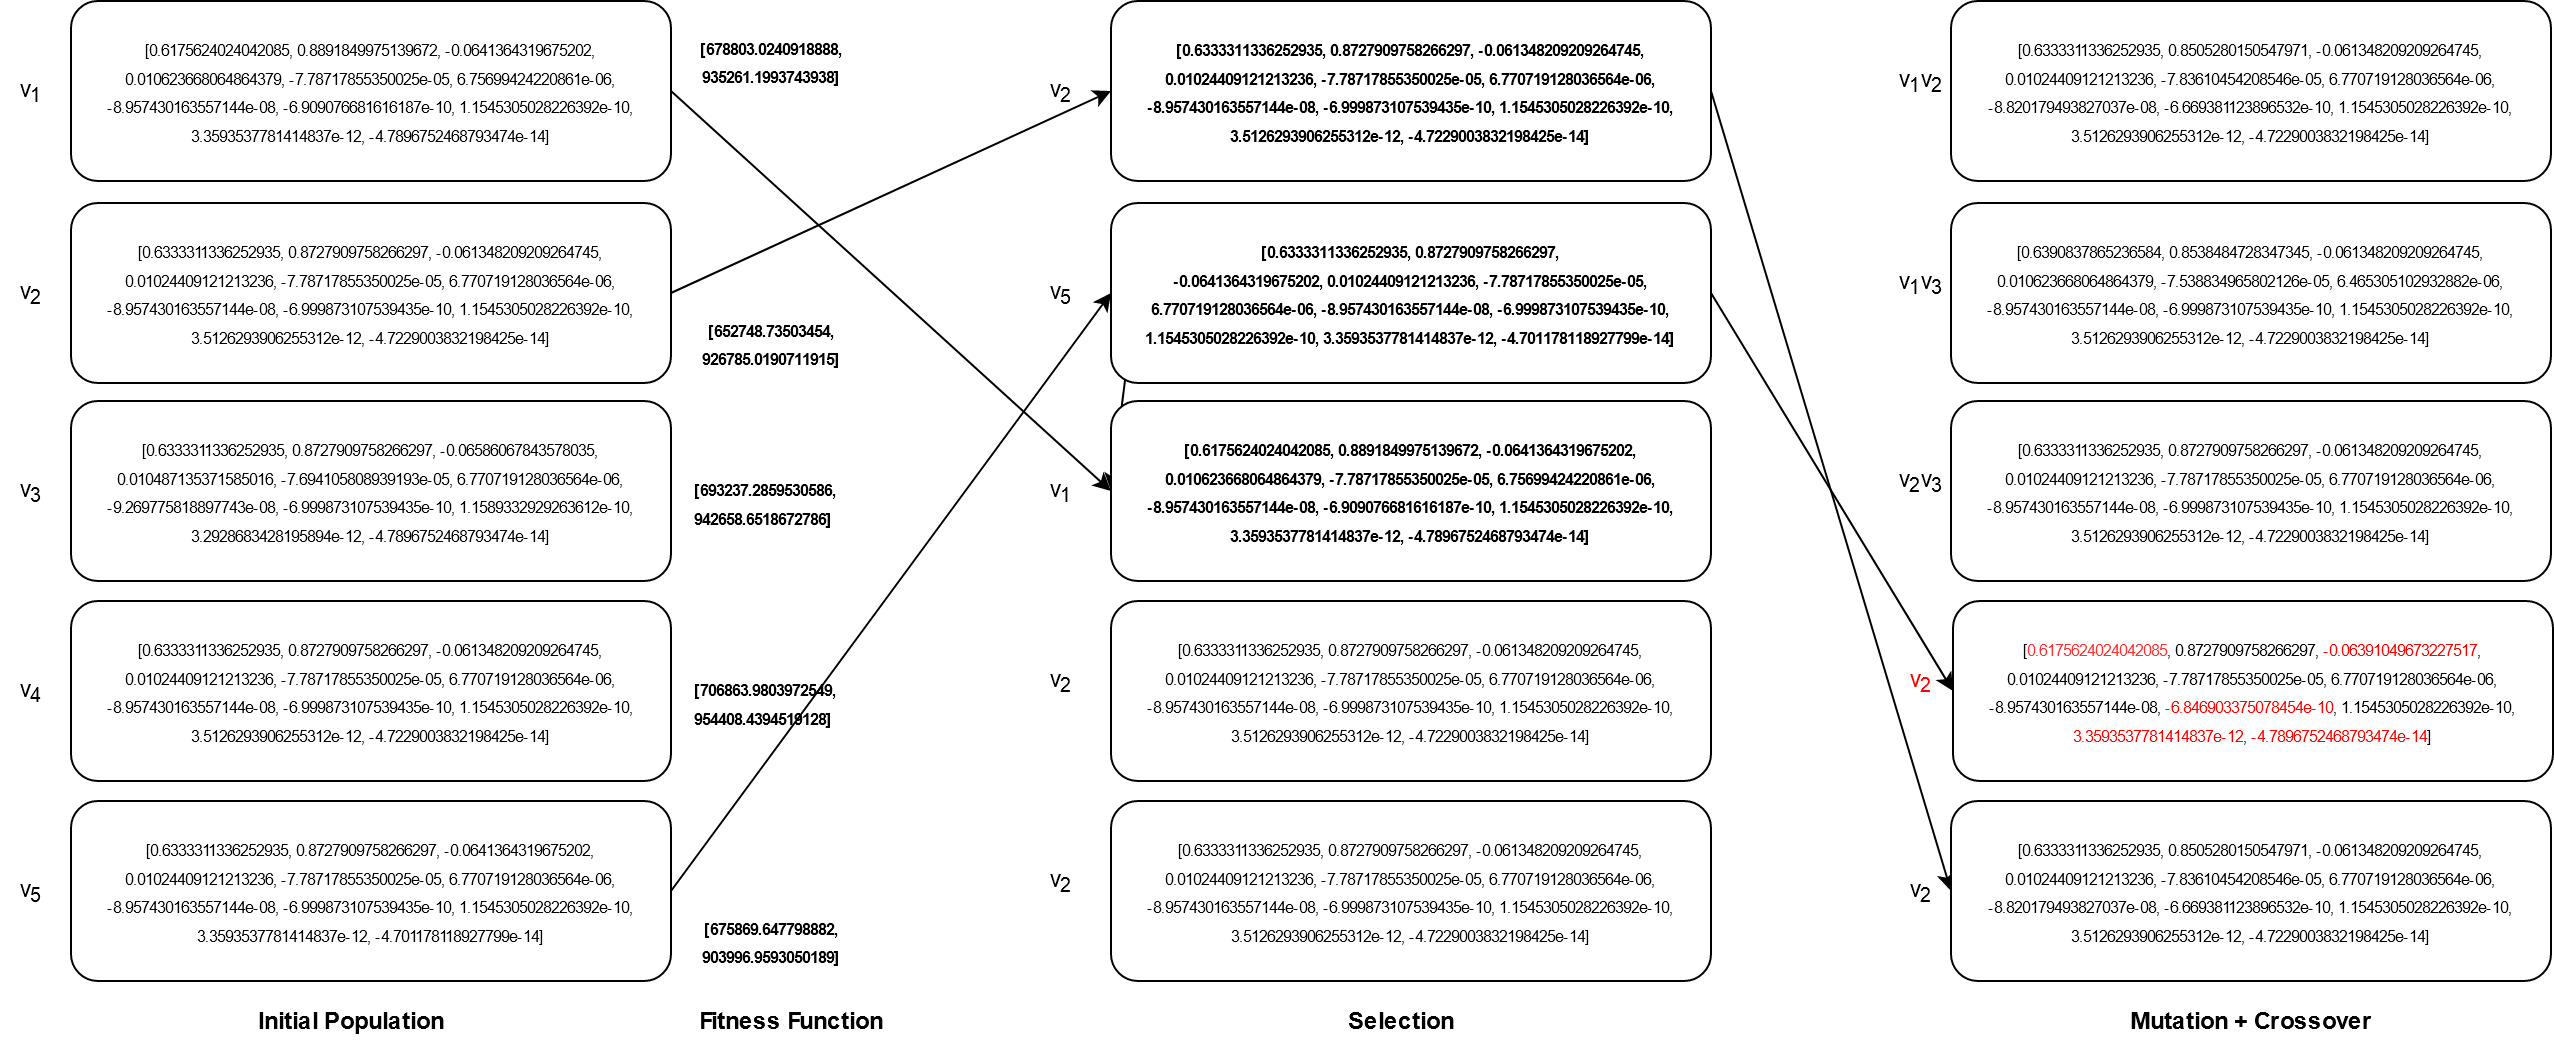
\includegraphics[width=\linewidth]{iteration1.jpg}
		\\
		\textit{iteration1.jpg}
	  \end{center}
	  \begin{center}
		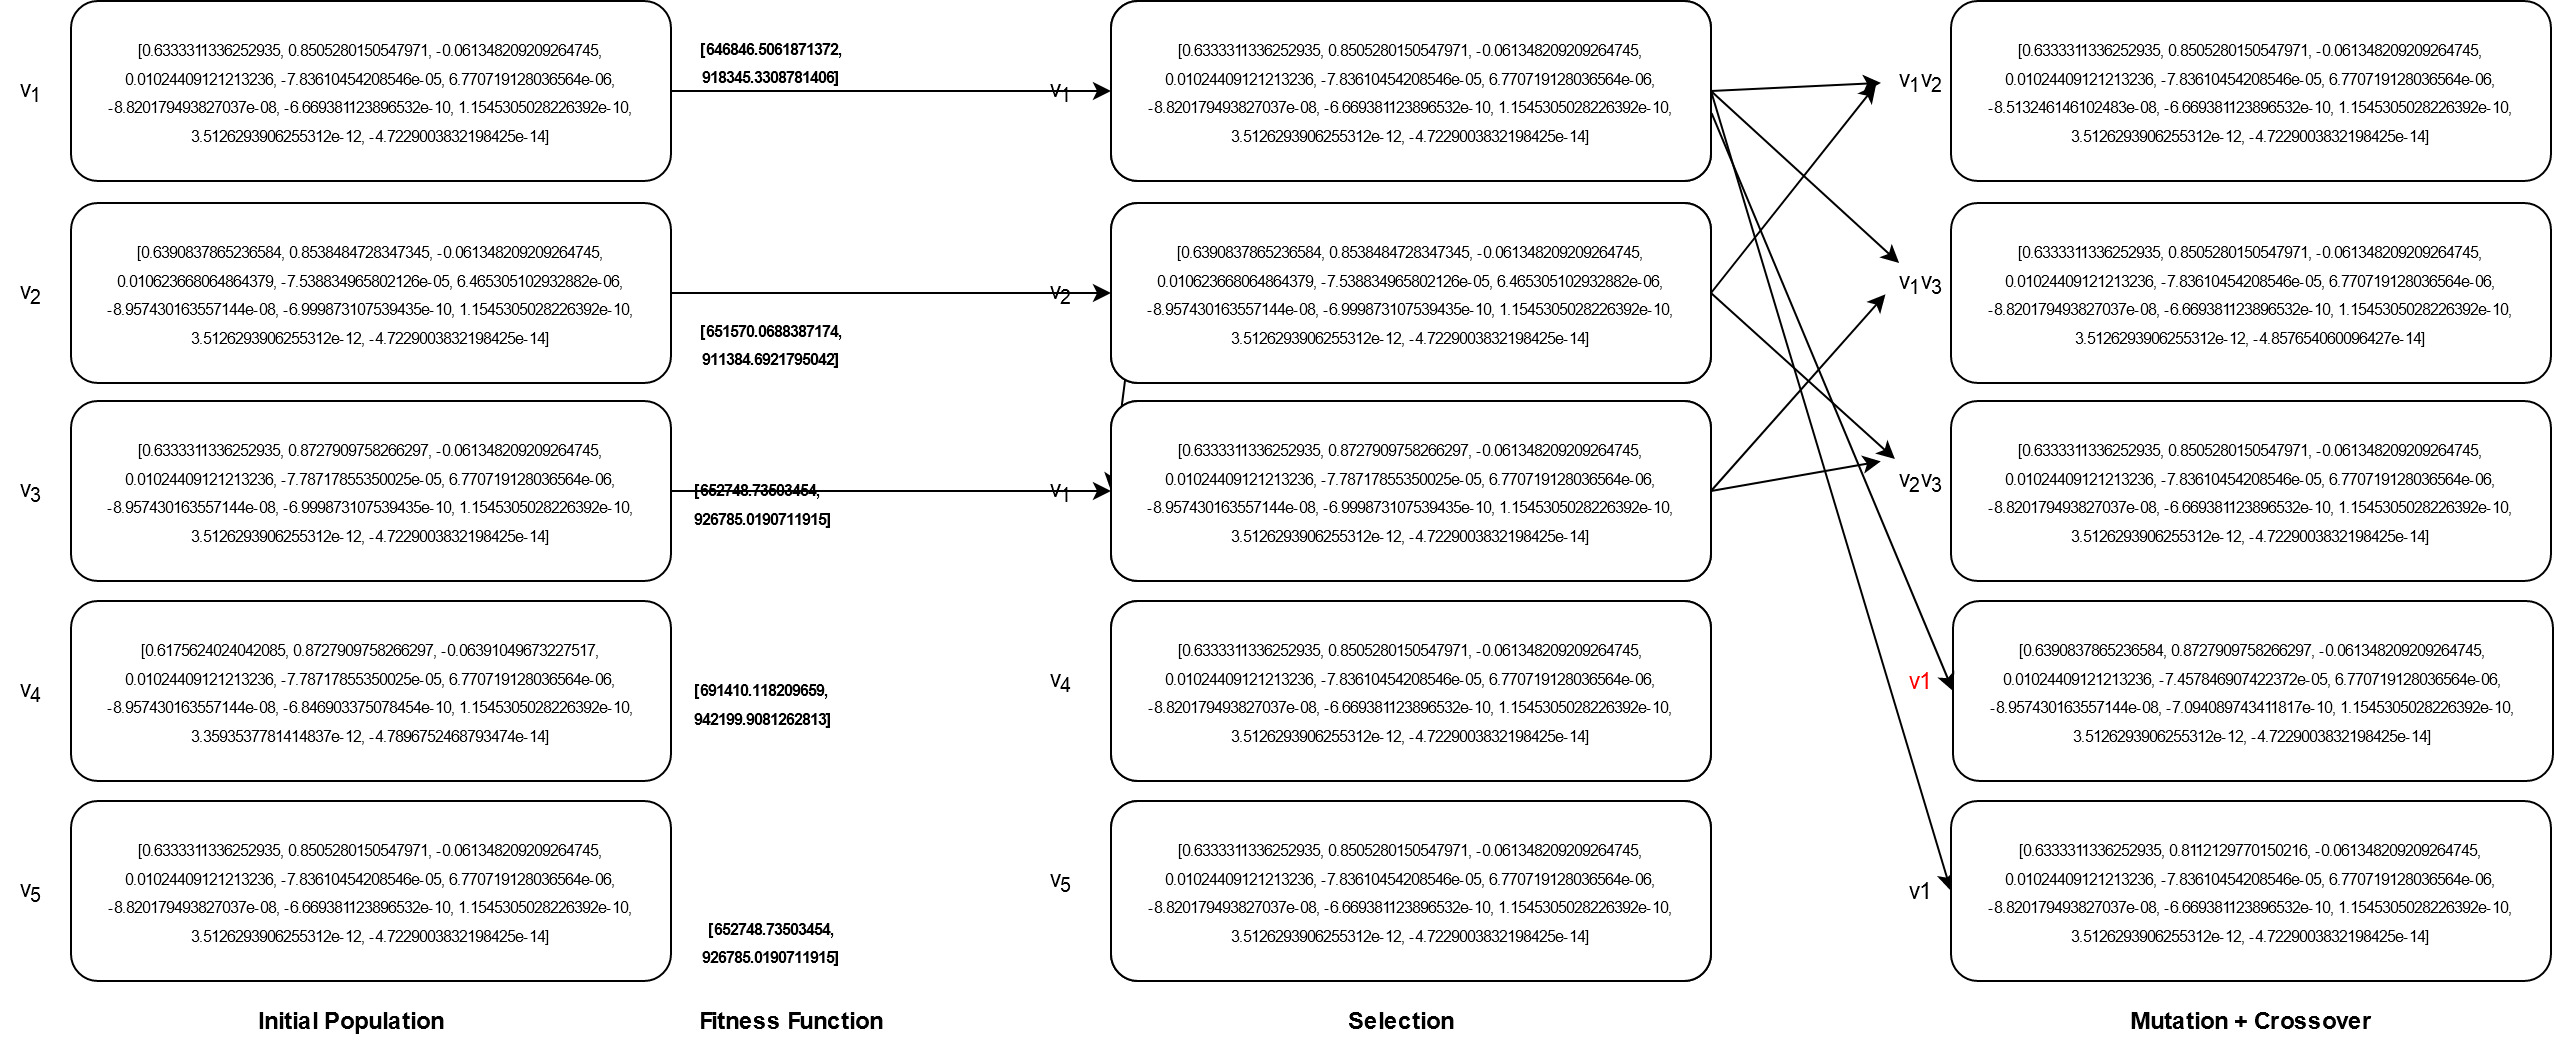
\includegraphics[width=\linewidth]{iteration2.jpg}
		\\
		\textit{iteration2.jpg}
	  \end{center}
	  \begin{center}
		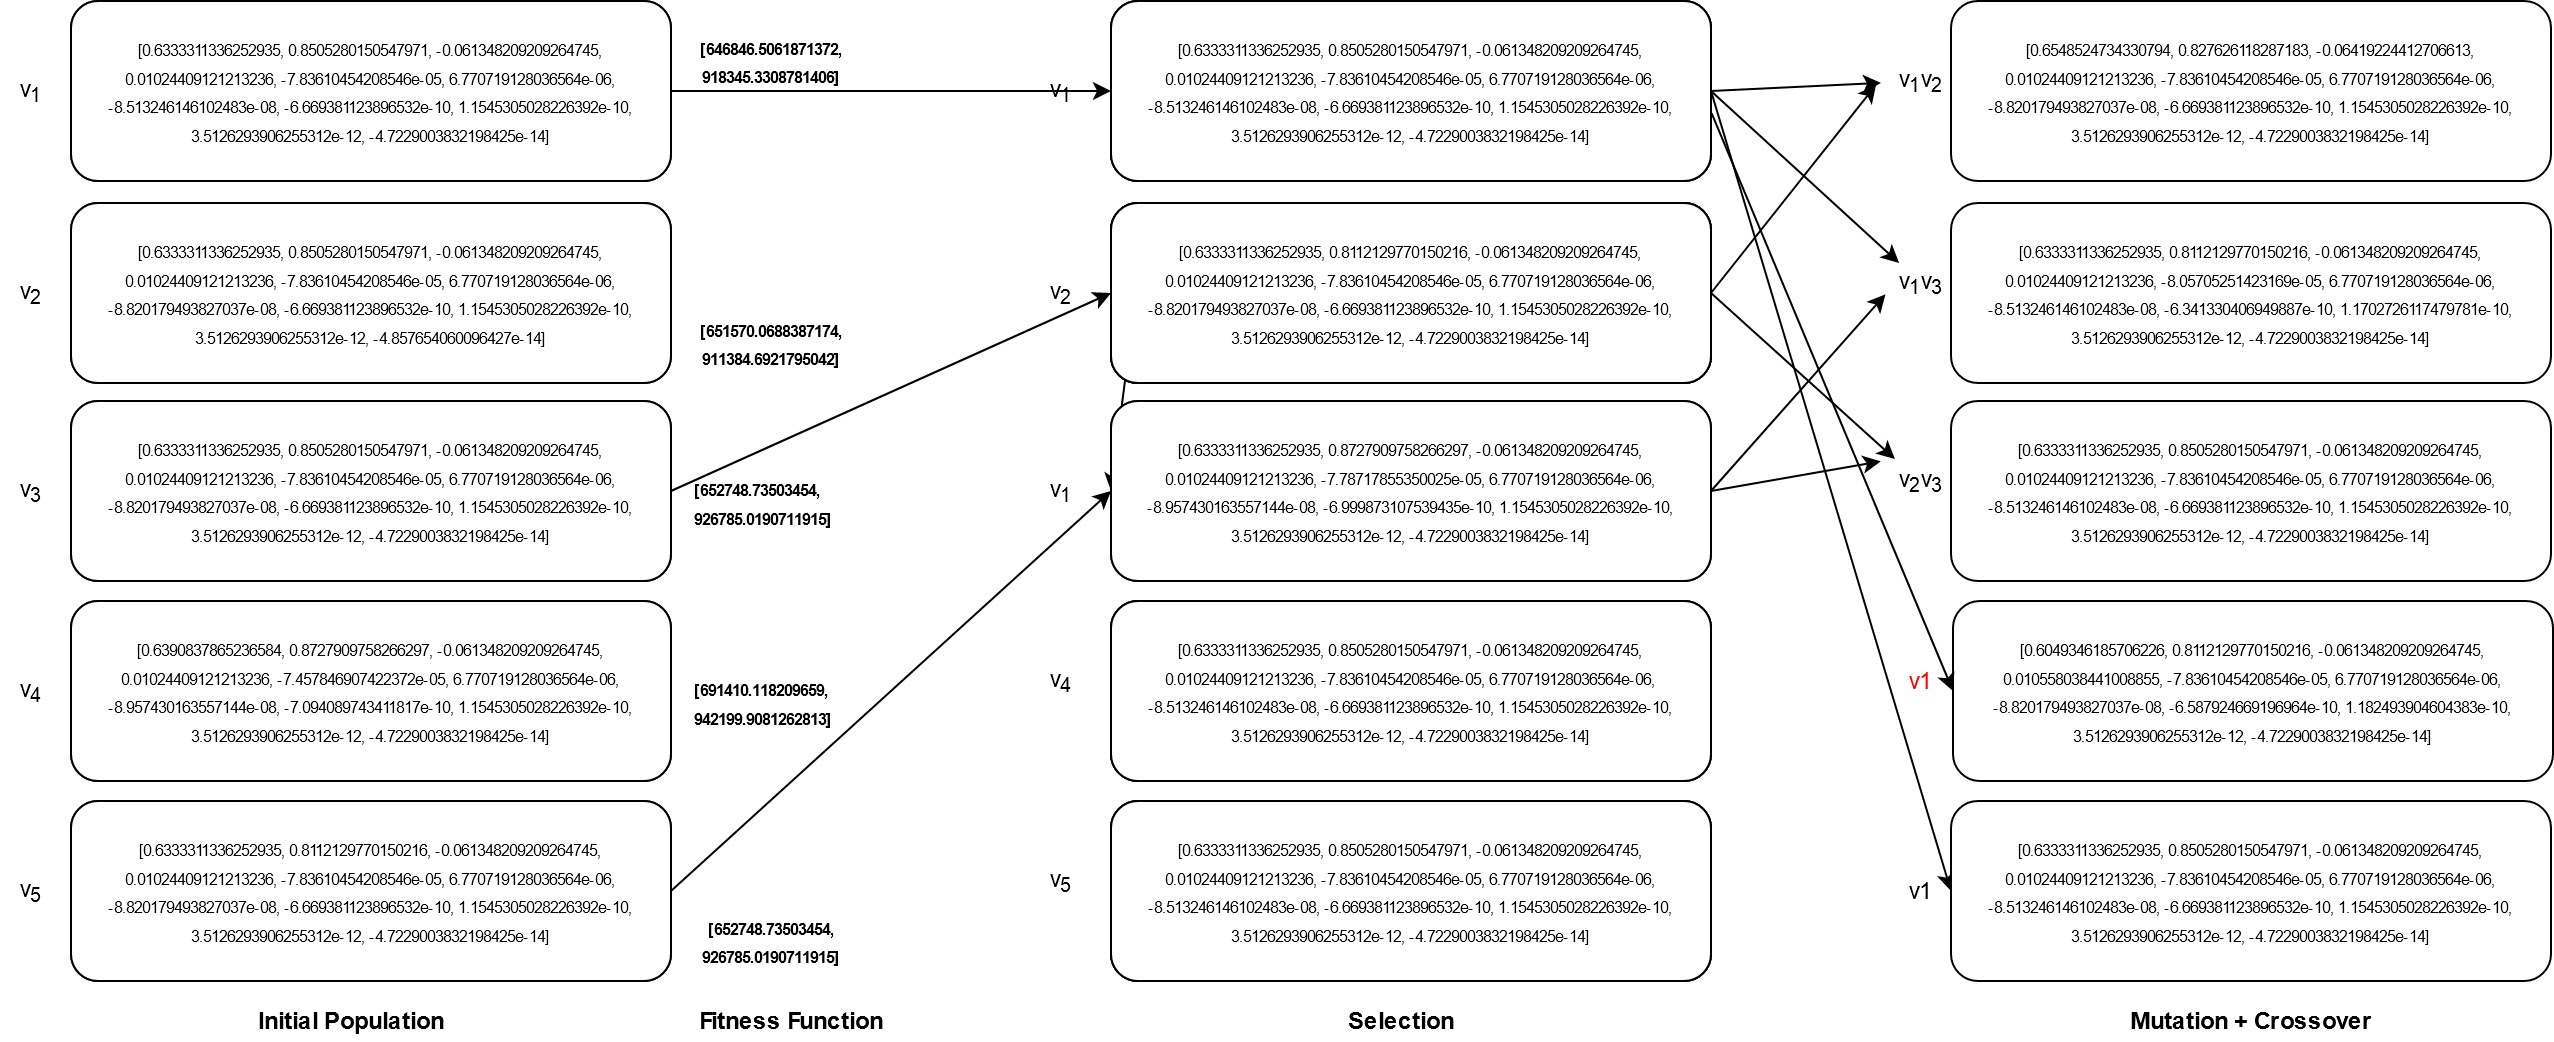
\includegraphics[width=\linewidth]{iteration3.jpg}
		\\
		\textit{iteration3.jpg}
	  \end{center}
	  The heuristics
	  We did a probabilistic cross over which is
	  explained above.
	  We introduced the concept of
	  survivability
	  The best vector always survive.
	  The best vector also produces a copy of
	  itself with some mutations.
	  This helps in converging towards a
	  minimum.
	  Also as the error becomes less we did a
	  trick.
	  (A-B)[0] survives only if it is better
	  than vector of previous generation.

\end{document}

